This chapter evaluates proceeding from the baseline to the implemented solution. Information about
server specifications (called Frodo) are provided in Table \ref{table:frodo-specs}, and information about the SmartNIC specifications are provided in Table \ref{table:smartnic-specs}. Experiments could be make thanks to \acrfull{npf} \cite{barbette_tbarbettenpf_2026}.

\section{Expiremental methodology}

\begin{table}[htpb]
    \centering
    \caption{Frodo server specifications}
    \label{table:frodo-specs}
    \small
    \begin{tabularx}{\columnwidth}{@{}lX@{}}
    \toprule
    \textbf{OS} & Ubuntu 22.04.5 LTS \\
    \textbf{Kernel} & 5.15.0-177-generic \\
    \textbf{CPU} & Intel(R) Xeon(R) E-2378 CPU @ 2.60GHz (16 cores) \\
    \textbf{RAM} & 2x 16 GB  DDR4 3200 MHz \\
    \textbf{Disks} & 2x SOLIDIGM SSDPFKKW010X7 (1TB) \\
    \textbf{NIC} & Mellanox ConnectX-6 (cf Table \ref{table:smartnic-specs}) \\
    \bottomrule
    \end{tabularx}
\end{table}

\begin{table}[htbp]
    \centering
    \caption{SmartNIC specification}
    \label{table:smartnic-specs}
    \begin{tabular}{@{}ll@{}}
        \toprule
        \textbf{Model} & Mellanox ConnectX-6 \\
        \midrule
        \textbf{OS} & Ubuntu 22.04.5 LTS \\
        \textbf{Kernel} & 5.15.0-1082-bluefield \\
        \textbf{CPU} & ARM Cortex-A72 (8 cores) \\
        \textbf{RAM} & 16 GB  DDR4 3200 MHz \\
        \textbf{NIC Speed} & 100 Gbps \\
        \bottomrule
    \end{tabular}
\end{table}

The evaluation methodology starts with a baseline of the disk performances, then evaluates the \acrshort{nvmeof} performance with Linux kernel. Next, we evaluate the performances of the original \texttt{lighttpd} version, and finally we evaluate the performances of IO-TCP implementation. Metrics are throughput, latency and CPU usage. The evaluation is made on Frodo server and on SmartNIC. Tools used for the evaluation are \texttt{\acrfull{fio}} \cite{noauthor_kernelgitaxboefiogit_nodate} for throughput and latency on disks, \texttt{wrk} \cite{glozer_wgwrk_2026} for throughput on \acrshort{http} server, and \texttt{perf} \cite{linux_perf,perfwiki} for CPU usage. 

Several parameters can influence the results of the evaluation. The first one is file / payload size, which means the size of the file to read or write on disk, or the size of the payload to send over the network. The second one is block size : the amount of data transferred in a single \acrshort{io} operation. Small block size (e.g 4 kB, the typical page and filesystem granularity) exercices the per request overhead of the \acrshort{io} stack (syscall, block layer, etc.) while large block size (e.g 4 MB) amortizes the overhead over many bytes, and is more representative of the disk raw transfer bandwidth capability. We therefore expect throughput to increase with block size up to the device or \acrshort{pcie} link bandwidth limit. The third one is \acrshort{io} depth, which is the number of \acrshort{io} operations that can be submitted to the device before waiting for completion. A higher \acrshort{io} depth allows for better utilization of the device and can improve throughput.. Throughput is expected to increase with \acrshort{io} depth, as well as latency due to queuing delays. The fourth one is the type of \acrshort{io} operation, which can be sequential or random read/write. Sequential operations are expected to have higher throughput and lower latency than random operations. The fifth one is the type of transport used for \acrshort{nvmeof}, which can be \acrshort{tcp} or \acrshort{rdma}. \acrshort{rdma} is expected to have lower latency and higher throughput than \acrshort{tcp} due to its direct memory access capabilities. Table \ref{table:workload-summary} shows the summary of the workloads.

\subsection{Tools parameters}

\texttt{\acrshort{fio}} is used to benchmark the disk throughput and latency. It can use different engines to submit \acrshort{io} operations. In this evaluation, we will use \texttt{libaio} \cite{libaio}, a standard Linux kernel asynchronous \acrshort{io} engine, \texttt{io\_uring} \cite{io_uring_manpage,what_is_io_uring}, a newer Linux kernel asynchronous \acrshort{io} interface, and \texttt{spdk\_bdev} \cite{spdk_bdev_user_guide}, a user-space library that bypasses the kernel and directly accesses the device. \texttt{libaio} and \texttt{io\_uring} are kernel-path engines, while \texttt{spdk\_bdev} is a user-space engine. For \texttt{spdk\_bdev}, we use an adapted implementation of \texttt{\acrshort{fio}} \cite{spdk_fio_bdev_readme} to benchmark metrics. 


\subsection{Workload summary}

\section{Disks performances baseline}

The first step in the measurements process is to evaluate the \acrfull{io} baseline performances of the disks, with and without \acrshort{spdk}. The first disk is connected to a \acrshort{pcie} 4.0 slot. We will call it disk A. The second disk is connected to a \acrshort{pcie} 3.0 slot. We will call it disk B.
Specifications of the disks are given in Table \ref{table:disk-specs}. The disks are SOLIDIGM SSDPFKKW010X7. Vendor theoretical speed are found in \cite{solidigm_2026,solidigm_benchmark_nodate,ssdpfkkw010x7x1performance_nodate}. The disks are connected to a \acrshort{pcie} 4.0 x4 and \acrshort{pcie} 3.0 x4 slot respectively. The submission queue is set to 64 bytes and the completion queue is set to 16 bytes. The maximum number of requests is set to 1023. Information about submission queue, completion queue and maximum number of requests have been collected with \texttt{nvme-cli} \cite{noauthor_linux-nvmenvme-cli_2026}.

In the following subsections \ref{subsec:disk-throughput} and \ref{subsec:disk-latency}, we will benchmark the throughput and latency of the disks with different file size, block size and \acrshort{io} depth. This will give us a baseline to compare with the implementation of \acrshort{nvmeof}, \acrshort{spdk}, and finally \textbf{IO-TCP}.

\begin{table}[htbp]
    \centering
    \caption{Disk specifications~\cite{solidigm_2026,solidigm_benchmark_nodate,ssdpfkkw010x7x1performance_nodate,noauthor_linux-nvmenvme-cli_2026}}
    \label{table:disk-specs}
    \begin{tabularx}{\columnwidth}{@{}l >{\raggedright\arraybackslash}X@{}}
        \toprule
        \textbf{Model} & SOLIDIGM SSDPFKKW010X7 (P44 Pro, 1\,TB) \\
        \midrule
        \textbf{PCIe slot} & Disk A: PCIe 4.0 $\times$4; Disk B: PCIe 3.0 $\times$4 \\
        \textbf{Sequential read (vendor)} & 7000 MB/s \\
        \textbf{Sequential write (vendor)} & 6500 MB/s \\
        \textbf{Submission queue entry} & 64 bytes \\
        \textbf{Completion queue entry} & 16 bytes \\
        \textbf{\texttt{nr\_requests}} & 1023 \\
        \bottomrule
    \end{tabularx}
\end{table}


\nt{You need to explain stuff more, what is depth, what is block size, how do you expect them to behave, how do they actually behave?}
\nt{I think overall profiling is missing to understand why one is fater than the other}
\subsection{Throughput} \label{subsec:disk-throughput}

% TO-DO : mention data availability on the repository

Throughput has been evaluated on disk A for different file size, block size and \acrshort{io} depth. \acrshort{io} queue depth is set to 64. Block size is set to 4kB and 4MB. File size is set to 4MB, 10MB, 100MB and 1GB. For each configuration, we run 5 times the test and we compute the mean, standard deviation, minimum, median and maximum throughput. Tests are time-based over 10 seconds, with a ramp time (warming up) of 3 seconds. The results are summarized in tables \ref{tab:stats-bandwidth-4K}, \ref{tab:stats-bandwidth-4M}, and \ref{tab:stats-write-bandwidth-4K}, and \ref{tab:stats-write-bandwidth-4M}. The figures \ref{fig:read-bandwidth-4K}, \ref{fig:read-bandwidth-4M}, \ref{fig:write-bandwidth-4K} and \ref{fig:write-bandwidth-4M} show the throughput of sequential read and write operations with 4kB and 4MB block size respectively. Finally, we ran a time-based test of 300 seconds and ramp time of 30 seconds to evict eventual SLC caching in subsection \ref{subsec:slc-caching}.


\subsubsection{Sequential read}
\nt{This is very dense, try to make it readable and list the main takeaways at the end}

Figure \ref{fig:read-bandwidth-4K} depicts the throughput over 4 kilobytes block size. At small file size (4MB and 10MB), kernel-path engines are bottlenecked and far behind device bandwidth, while \acrshort{spdk} achieves systemically higher throughput. \acrshort{spdk} deliver up to 4.5 times higher throughput than kernel-path engines. The standard deviation of \acrshort{spdk} is also significantly lower than kernel-path engines, ranging from 313.99 kB/s to 10.7 MB/s while kernel-path engines range from 33.50 MB/s to 61.94 MB/s. At larger file size (100MB and 1GB), \acrshort{spdk} is still ahead of kernel-path engines, but the throughput remains 0.8 times \nt{(1.8?)} higher. The standard deviation of \acrshort{spdk} is yet again significantly lower than kernel-path engines, ranging from 1.49 MB/s to 12.46 MB/s while kernel-path engines range from 41.52 MB/s to 55.04 MB/s. The results are summarized in table \ref{tab:stats-bandwidth-4K}. The reason why \acrshort{spdk} performs better than kernel-path engines is that \acrshort{spdk} bypasses the kernel and directly accesses the device, while kernel-path engines have to go through the kernel, which adds overhead.~\nt{You need to better detail the mechanism} 
% Explain why kernel perfoms better at large file than small file.
% Run perf 
% Tests with multiple threads / cores

\begin{figure}[htbp]
    \centering
    \begin{minipage}{0.495\columnwidth}
        \centering
        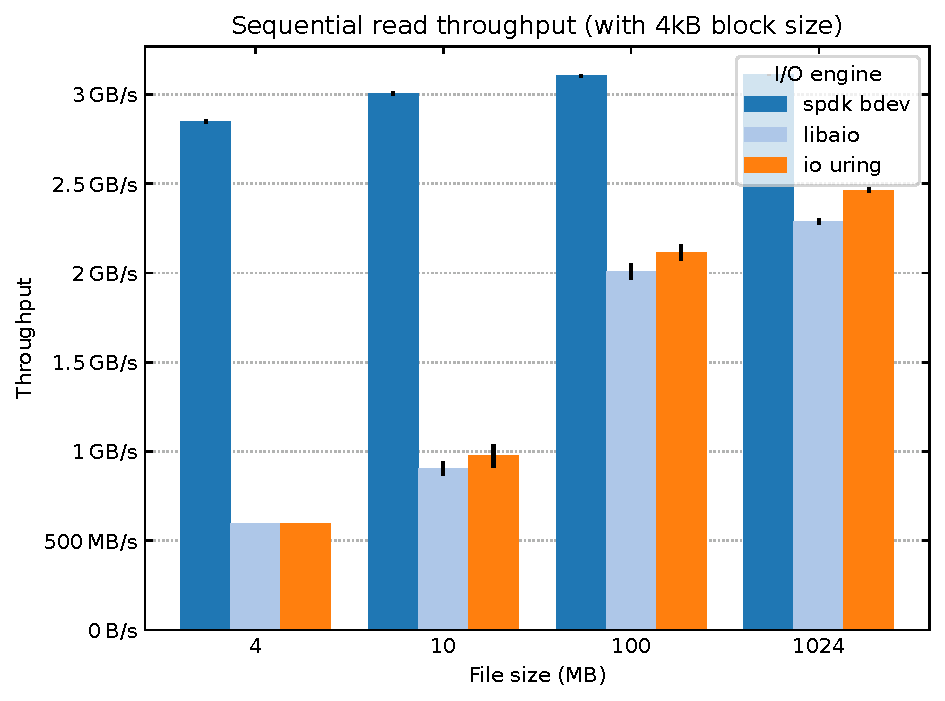
\includegraphics[width=\linewidth]{../measurements/npf/experiments/spdk/bs-4K/graphs/read-BANDWIDTH.pdf}
        \caption{Throughput of sequential read operations with 4kB block size}
        \label{fig:read-bandwidth-4K}
    \end{minipage}
    \hfill
    \begin{minipage}{0.495\columnwidth}
        \centering
        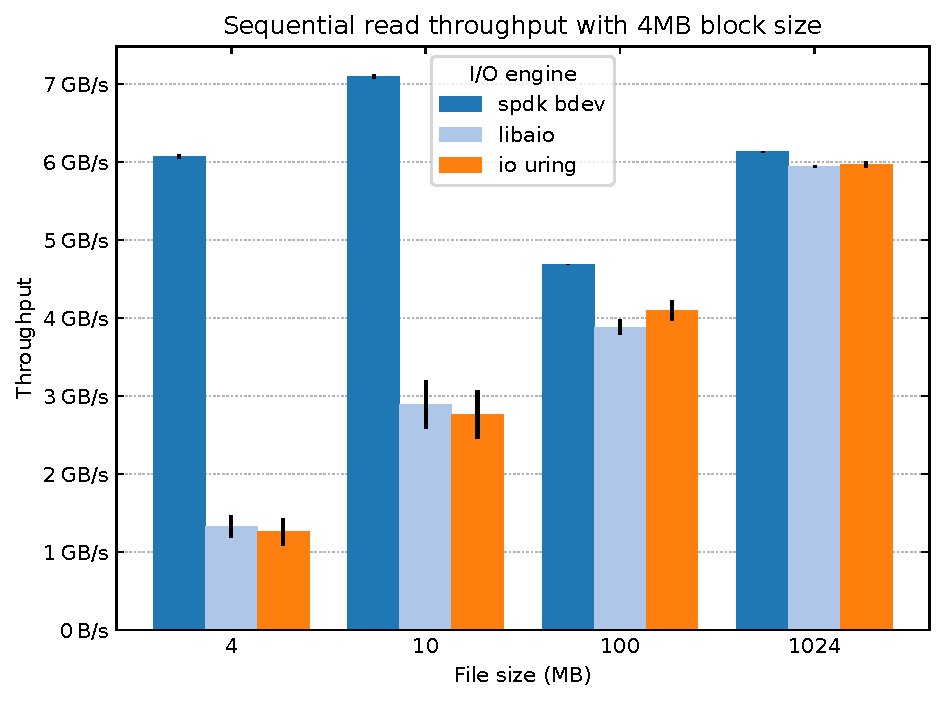
\includegraphics[width=\linewidth]{../measurements/npf/experiments/spdk/bs-4M/graphs/read-BANDWIDTH.pdf}
        \caption{Throughput of sequential read operations with 4MB block size}
        \label{fig:read-bandwidth-4M}
    \end{minipage}
\end{figure}

Looking at figure \ref{fig:read-bandwidth-4M} which illustrates throughput with 4 megabytes block size, we can observe that througput of all engines increase compared to 4kB block size. \acrshort{spdk} is consistent for all file size, with an average throughput of 6.73 GB/s (maximum achived is 6.75 GB/s). This throughput is close to the vendor theoretical speed of 7 GB/s. Kernel-path engines are still bottlenecked at small file size (4MB and 10MB), with an average throughput of respectively 1.53 GB/s and 2.01 GB/s, thus making \acrshort{spdk} 4.4 times faster than kernel-path engines. At larger file size (100MB and 1GB), kernel-path engines are able to achieve a mean throughput of 3.31 GB/s and 5.43 GB/s respectively, thus making \acrshort{spdk} 1.24 to 2.03 times faster than kernel-path engines. Standard deviation of \acrshort{spdk} is also significantly lower than kernel-path engines, ranging from 11.97 MB/s to 16.74 MB/s while kernel-path engines range from 96.58 MB/s to 218.24 MB/s. The results are summarized in table \ref{tab:stats-bandwidth-4M}.

We can conclude that \acrshort{spdk} is able to achieve higher throughput for sequential read operations with lower standard deviation than kernel-path engines, especially at small file size. It also follows the same order of magnitude for small file size regardless of block size, and is able to achieve close to vendor theoretical speed with large block size.


\subsubsection{Sequential write}

For sequential write with block size of 4 kB (figure \ref{fig:write-bandwidth-4K}), we can observe that \acrshort{spdk} is more stable in its mean output, reaching 6.25 GB/s with standard deviation of 35.09 MB/s to 59.09 MB/s. Kernel-path engines are capped at 2.1 GB/s in their best case, with standard deviation of 35.37 MB/s to 353.55 MB/s. Unlike read operations, write operations are bounded by the device NAND program time rather than \acrshort{pcie} bandwidth, so these numbers must also account eventual SLC caching. The results are summarized in table \ref{tab:stats-write-bandwidth-4K}.

\begin{figure}[htbp]
    \centering
    \begin{minipage}{0.495\columnwidth}
        \centering
        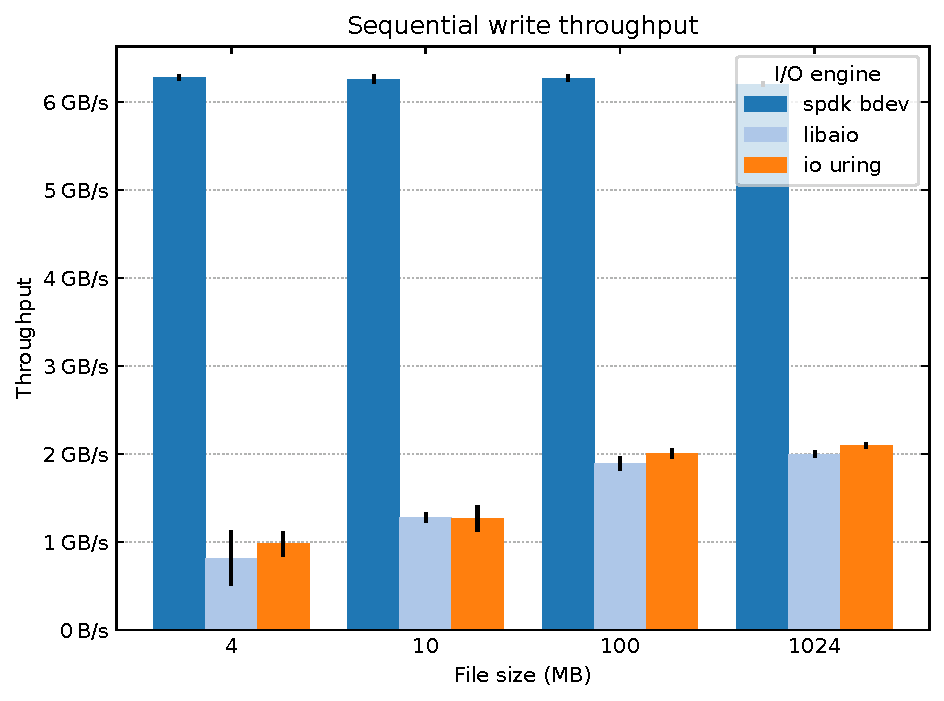
\includegraphics[width=\linewidth]{../measurements/npf/experiments/spdk/bs-4K/graphs/write-BANDWIDTH.pdf}
        \caption{Throughput of sequential write operations with 4kB block size}
        \label{fig:write-bandwidth-4K}
    \end{minipage}
    \hfill
    \begin{minipage}{0.495\columnwidth}
        \centering
        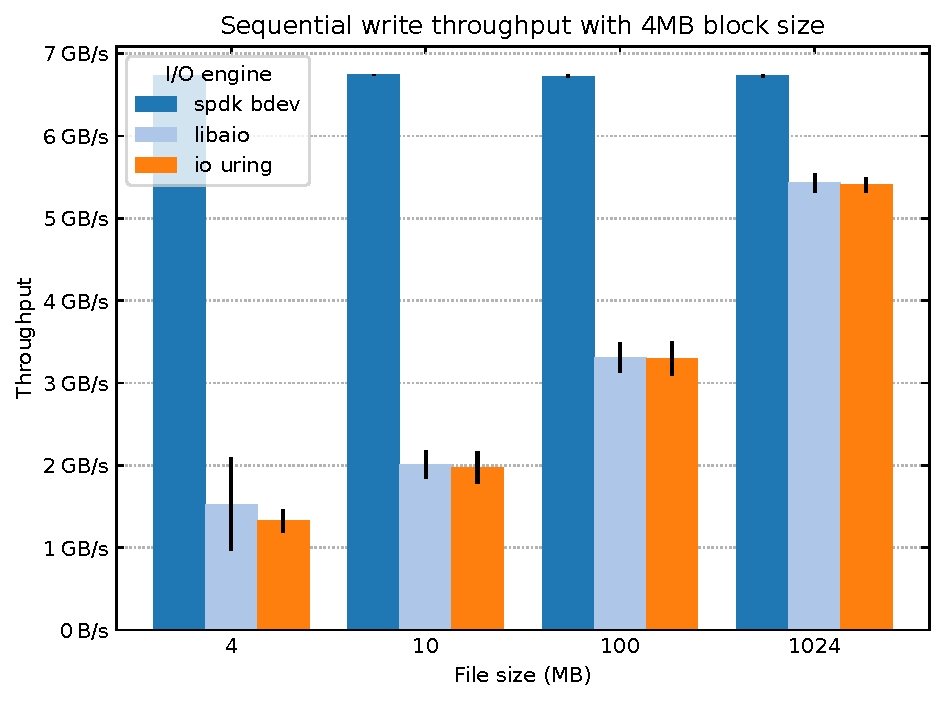
\includegraphics[width=\linewidth]{../measurements/npf/experiments/spdk/bs-4M/graphs/write-BANDWIDTH.pdf}
        \caption{Throughput of sequential write operations with 4MB block size}
        \label{fig:write-bandwidth-4M}
    \end{minipage}
\end{figure}

Figure \ref{fig:write-bandwidth-4M} shows the throughput of sequential write operations with 4MB block size. At this block size, \acrshort{spdk} has an higher average throughput of 6.73 GB/s with standard deviation of 11.97 MB/s to 16.74 MB/s, while kernel-path engines are capped at 5.43 GB/s with standard deviation of 96.58 MB/s to 595.86 MB/s.

While some configurations are able to exceed the vendor theoretical speed of 6.5 GB/s, caution should be taken as even if not specified by the vendor, the disk can use a dynamic \acrshort{pslc} write cache to achieve higher throughput. This is why we ran a time-based test of 300 seconds and ramp time of 30 seconds to evict eventual SLC caching in subsection \ref{subsec:slc-caching}.

\subsubsection{Random read and write}

    TO-DO

\subsection{Cost per I/O operation}

    Previous results show that kernel-path engines are impacted by the block size. We can compute the \acrfull{iops}  by dividing the throughput by the block size. Below is a table summarizing the average \acrshort{iops} for previous tests. The results show that \acrshort{spdk} is able to achieve higher \acrshort{iops} than kernel-path engines, especially at small block size. This is due to the fact that \acrshort{spdk} bypasses the kernel and directly accesses the device, while kernel-path engines have to go through the kernel, which adds overhead.

    \begin{table}[htbp]
        \centering
        \caption{Average \acrshort{iops} for all operations with 4kB and 4MB block size}
        \label{tab:stats-iops}
            \begin{tabularx}{\columnwidth}{@{}l l X X X@{}}
            \toprule
            \textbf{Block size} & \textbf{Operations} & \texttt{io\_uring} & \texttt{libaio} & \texttt{spdk\_bdev}\\
            \midrule
            \textbf{4kB} & Sequential Read & 397.03 kIOPS & 374.2 kIOPS & 1.56 MIOPS \\
            \textbf{4kB} & Random Read & 382.62 kIOPS & 355.03 kIOPS & 742.92 kIOPS \\
            \textbf{4kB} & Sequential Write & 397.03 kIOPS & 374.2 kIOPS & 1.56 MIOPS \\
            \textbf{4kB} & Random Write & 361.5 kIOPS & 339.55 kIOPS & 590.92 kIOPS \\
            \midrule
            \textbf{4MB} & Sequential Read & 384.53 IOPS & 362.57 IOPS & 753.92 kIOPS \\
            \textbf{4MB} & Random Read & 822.49 IOPS & 834.12 IOPS & 1.46 kIOPS \\
            \textbf{4MB} & Sequential Write & 750.63 IOPS & 767.51 IOPS & 1.68 kIOPS \\
            \textbf{4MB} & Random Write & 750.63 IOPS & 767.51 IOPS & 1.68 kIOPS \\
            \bottomrule
            \end{tabularx}
    \end{table}

    % \begin{figure}[htbp]
    %     \centering
    %     \begin{minipage}{0.495\columnwidth}
    %         \centering
    %         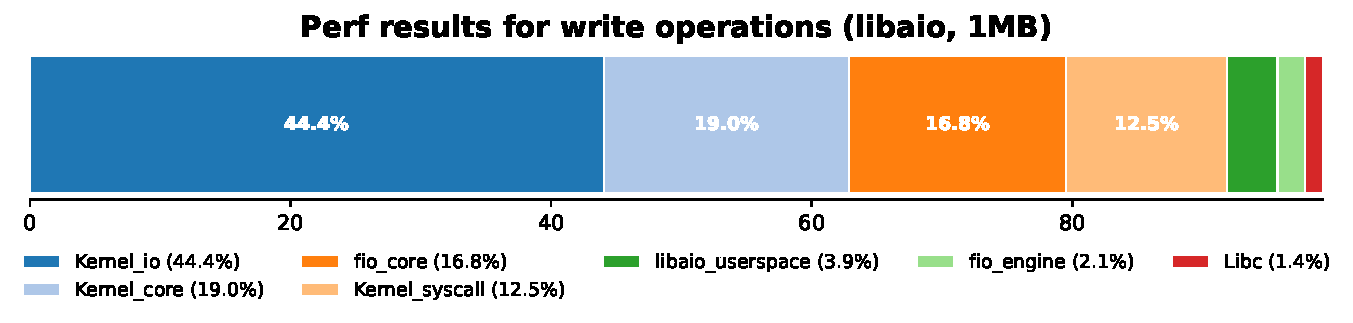
\includegraphics[width=\linewidth]{../measurements/perf/pdf/perf_libaio_write_20261028_154323.pdf}
    %         \caption{Perf of sequential write operations with 4kB block size and 1MB file size}
    %         \label{fig:perf-write-4k-1M}
    %     \end{minipage}
    %     \hfill
    %     \begin{minipage}{0.495\columnwidth}
    %         \centering
    %         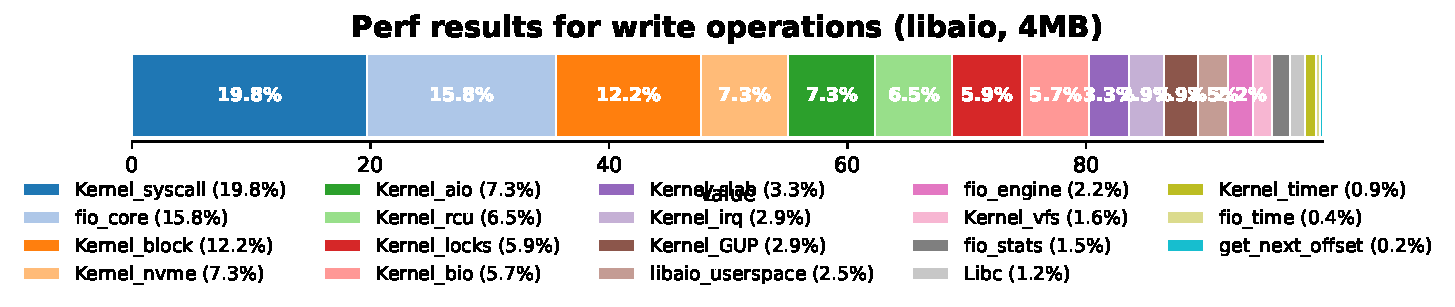
\includegraphics[width=\linewidth]{../measurements/perf/pdf/perf_libaio_4_write_20261028_171603.pdf}
    %         \caption{Throughput of sequential write operations with 4kB block size and 4MB file size}
    %         \label{fig:perf-write-4k-4M}
    %     \end{minipage}
    % \end{figure}
    \begin{figure}[htbp]
        \centering
        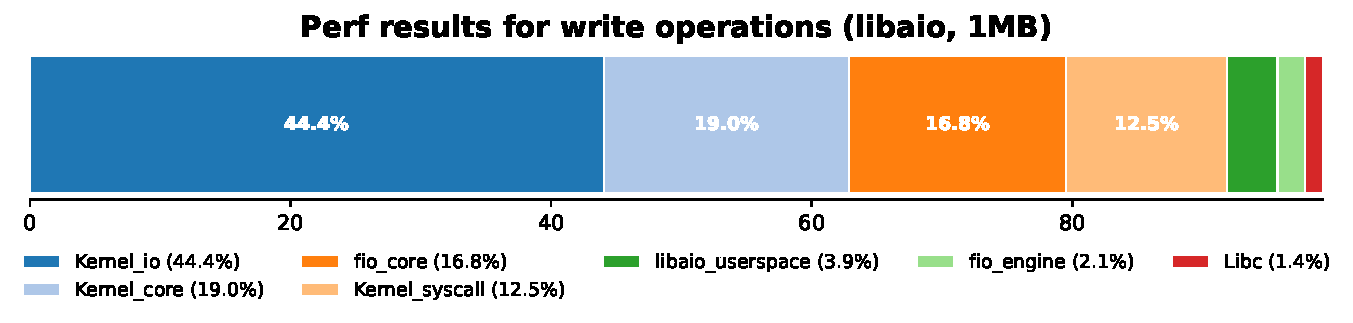
\includegraphics[width=\columnwidth]{../measurements/perf/pdf/perf_libaio_write_20261028_154323.pdf}
        \caption{Perf of sequential write operations with 4kB block size and 1MB file size with \texttt{libaio}}
        \label{fig:perf-write-libaio-4k-1M}
    \end{figure}

    \begin{figure}[htbp]
        \centering
        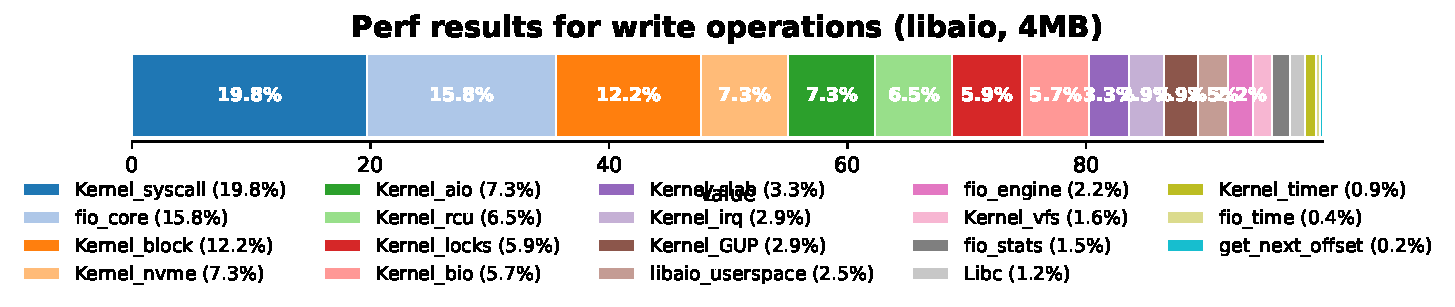
\includegraphics[width=\columnwidth]{../measurements/perf/pdf/perf_libaio_4_write_20261028_171603.pdf}
        \caption{Perf of sequential write operations with 4kB block size and 4MB file size with \texttt{libaio}}
        \label{fig:perf-write-libaio-4k-4M}
    \end{figure}

    \begin{figure}[htbp]
        \centering
        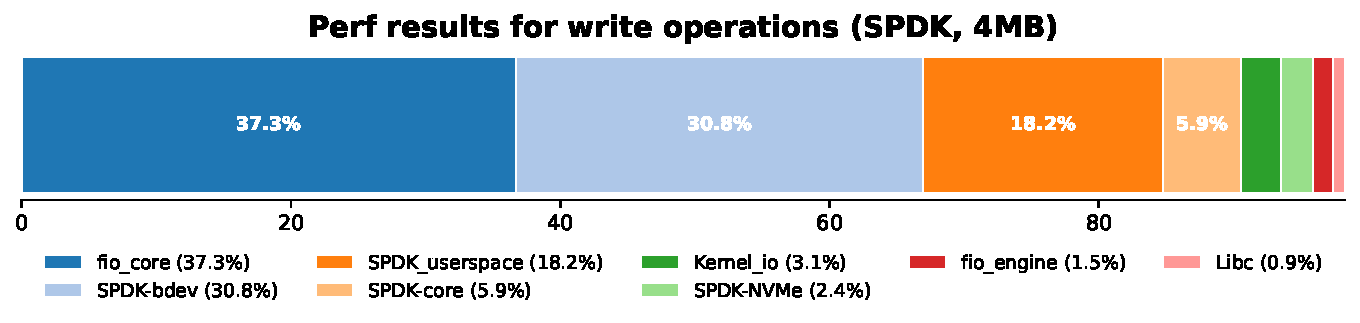
\includegraphics[width=\columnwidth]{../measurements/perf/bs-4K/pdf/perf_spdk_bdev_4_write_20261104_182456.pdf}
        \caption{Perf of sequential write operations with 4kB block size and 4MB file size with SPDK}
        \label{fig:perf-write-spdk-4k-4M}
    \end{figure}

    
    For example, for sequential read operations with 4kB block size, \acrshort{spdk} achieves on average 753.92 k\acrshort{iops} while kernel-path engines achieve on average 362.57 k\acrshort{iops} for \texttt{libaio} and 384.53 k\acrshort{iops} for \texttt{io\_uring}, nearly 2 times less. For 4MB block size, \acrshort{spdk} got on average 1.5 K\acrshort{iops} while \texttt{io\_uring} got 880.83 \acrshort{iops} and \texttt{libaio} got 878.34 \acrshort{iops}, nearly 1.7 times less.
    
    Figures \ref{fig:perf-write-4k-1M} and \ref{fig:perf-write-4k-4M} show the \texttt{perf} of sequential write operations with 4kB block size and 1MB or 4MB file size respectively. Up to 20 \% of the CPU time is spent on system calls. Detailed classification of the CPU time is available in table \ref{tab:perf-categories}.

\subsection{SLC cache} \label{subsec:slc-caching}

    TO-DO

    \begin{figure}[htbp]
        \centering
        \begin{minipage}{0.495\columnwidth}
            \centering
            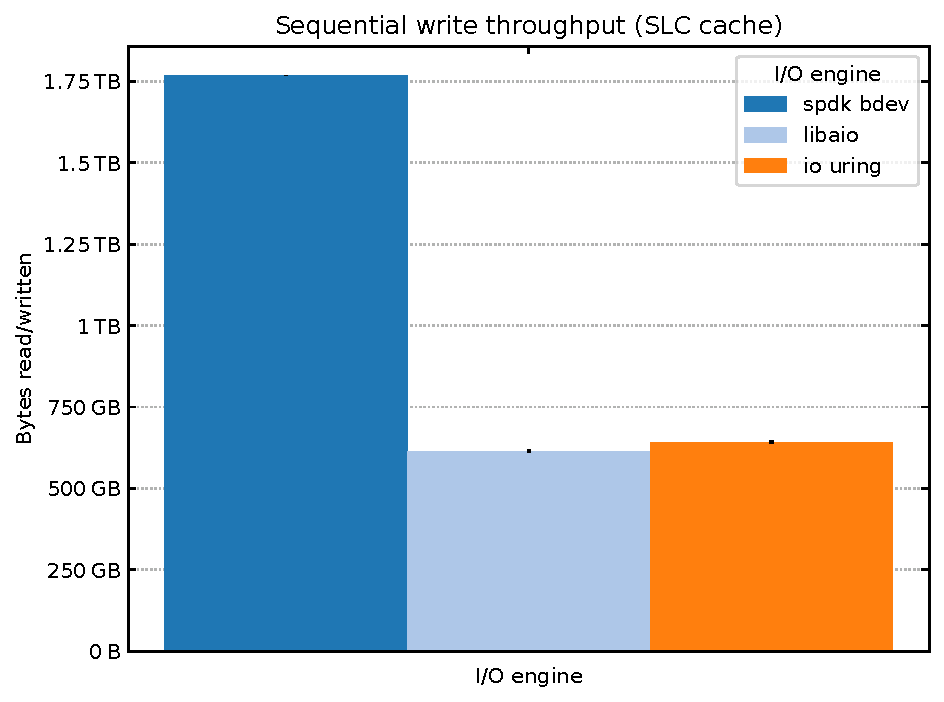
\includegraphics[width=\linewidth]{../measurements/npf/experiments/spdk/slc/graphs/write-IO_BYTES.pdf}
            \caption{Throughput of sequential write operations with 4kB block size and 1MB file size}
            \label{fig:slc-write-iobytes}
        \end{minipage}
        \hfill
        \begin{minipage}{0.495\columnwidth}
            \centering
            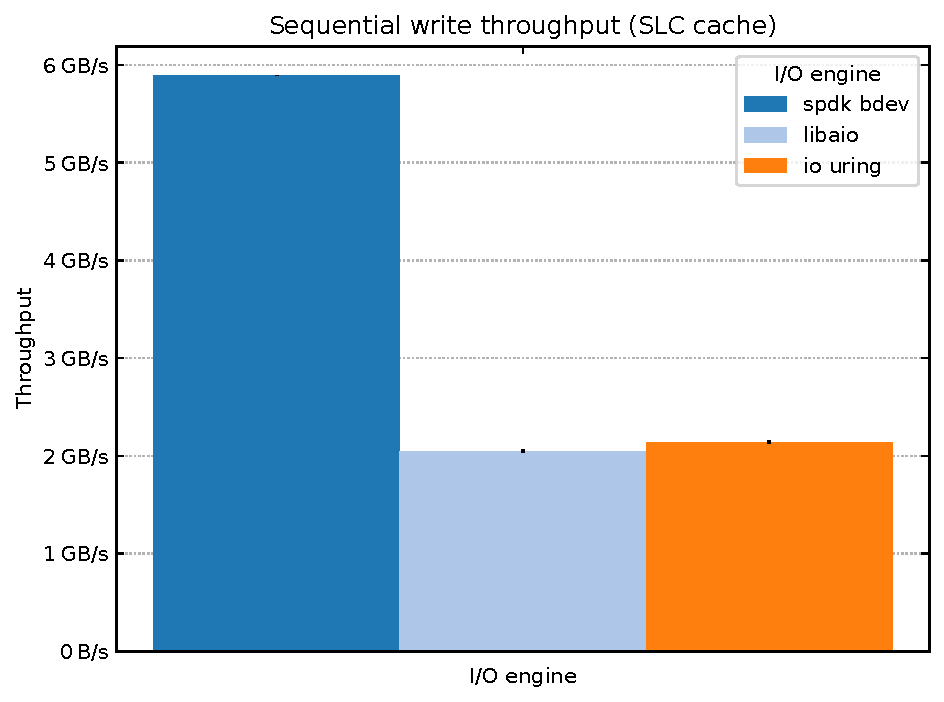
\includegraphics[width=\linewidth]{../measurements/npf/experiments/spdk/slc/graphs/write-BANDWIDTH.pdf}
            \caption{Throughput of sequential write operations with 4kB block size and 4MB file size}
            \label{fig:slc-write-bandwidth}
        \end{minipage}
    \end{figure}

\subsection{Latency} \label{subsec:disk-latency}

    TO-DO


\nt{Expland the discussion}
\subsection{Multiple cores} \label{subsec:disk-multicore}

    TO-DO
    
\section{NVMe-over-Fabrics performances}

    In this section we evaluate the throughput and latency of NVMe-over-Fabrics with Linux kernel on disk A. The tests evaluate both \acrshort{tcp} and \acrshort{rdma} transport. The tests are made with \texttt{\acrshort{fio}} \cite{noauthor_kernelgitaxboefiogit_nodate} with \texttt{io\_uring} engine. Queue depth is fixed to 64.

    \subsection{Throughput}

        \begin{figure}[htbp]
        \centering
        \begin{minipage}{0.495\columnwidth}
            \centering
            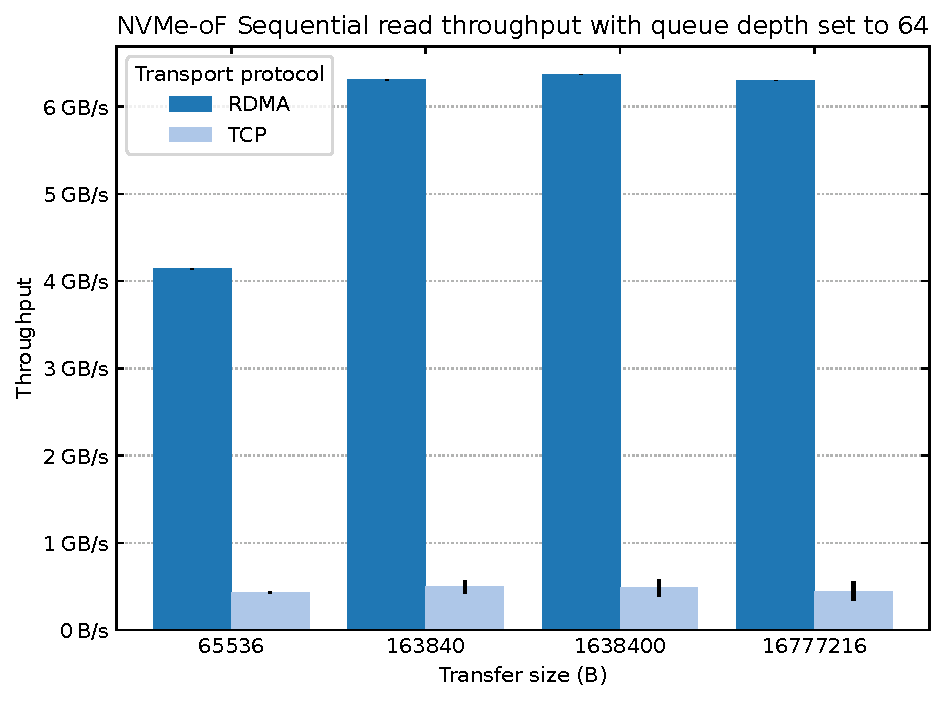
\includegraphics[width=\linewidth]{../measurements/npf/experiments/spdk/nvme-of/graphs/-read-BANDWIDTH.pdf}
            \caption{Throughput of sequential read operations for NVMe-over-Fabrics with large file size}
            \label{fig:nmve-of-read-bandwidth}
        \end{minipage}
        \hfill
        \begin{minipage}{0.495\columnwidth}
            \centering
            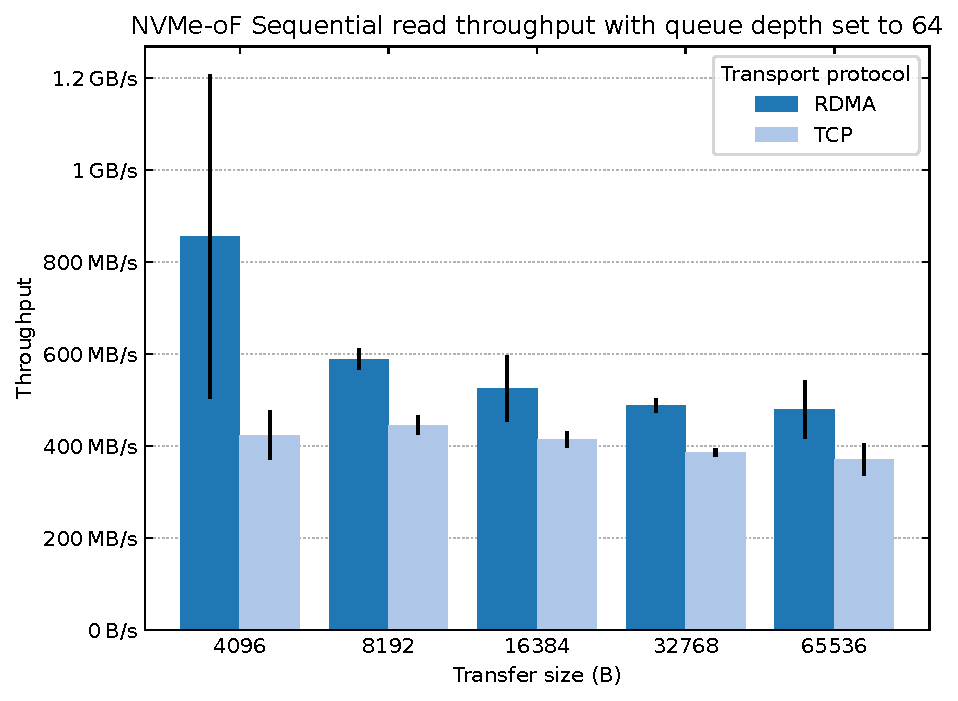
\includegraphics[width=\linewidth]{../measurements/npf/experiments/spdk/nvme-of/graphs/small-read-BANDWIDTH.pdf}
            \caption{Throughput of sequential read operations for NVMe-over-Fabrics with small file size}
            \label{fig:nmve-of-read-bandwidth-small}
        \end{minipage}
    \end{figure}

\section{lighttpd performances}

We benchmarked the \acrshort{http} server \texttt{lighttpd} original version (1.4.32) \cite{lighttpd_1.4.32_news,lighttpd_1.4.32_github} in order to analyze the difference between the original version and the IO-TCP version. The benchmark is made with \texttt{wrk} \cite{glozer_wgwrk_2026}. To be fair with IO-TCP, we restrict the \texttt{lighttpd} to a single core. Figures \ref{fig:lighttpd-x86} and \ref{fig:lighttpd-arm} show the throughput of \texttt{lighttpd} on Frodo server (x86\_64 core) and on SmartNIC (ARM Cortex-A72 core) respectively. We observe that a single core on Frodo is nearly able to saturate the disk bandwidth.

\begin{figure}[htbp]
    \centering
    \begin{minipage}{0.495\columnwidth}
        \centering
        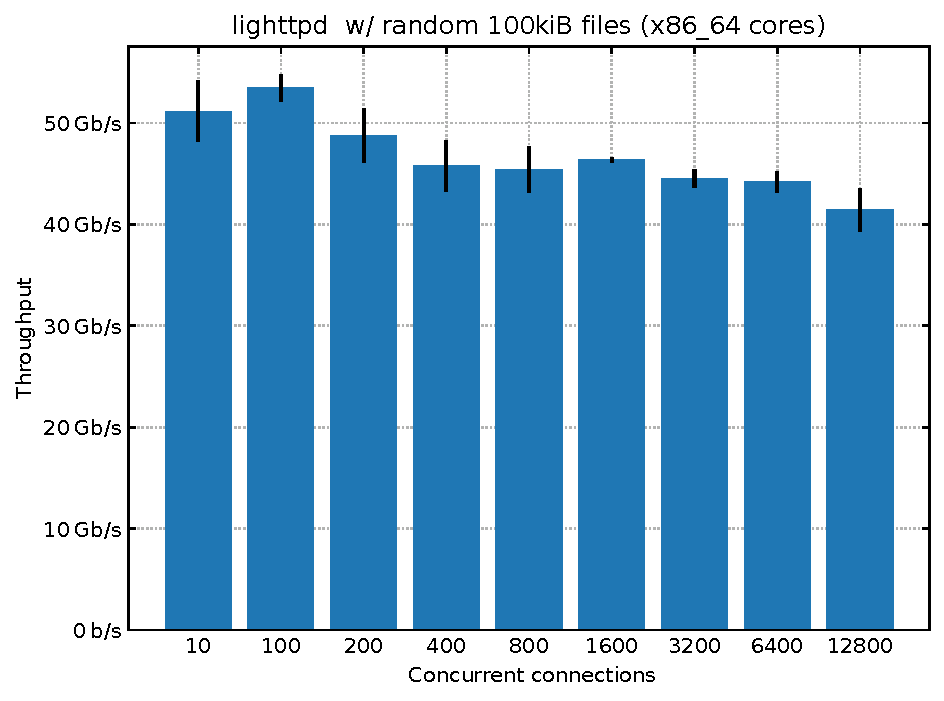
\includegraphics[width=\linewidth]{../measurements/npf/experiments/lighttpd/frodo-random-100k-BANDWIDTH.pdf}
        \caption{Throughput of lighttpd on Frodo server (x86\_64 core)}
        \label{fig:lighttpd-x86}
    \end{minipage}
    \hfill
    \begin{minipage}{0.495\columnwidth}
        \centering
        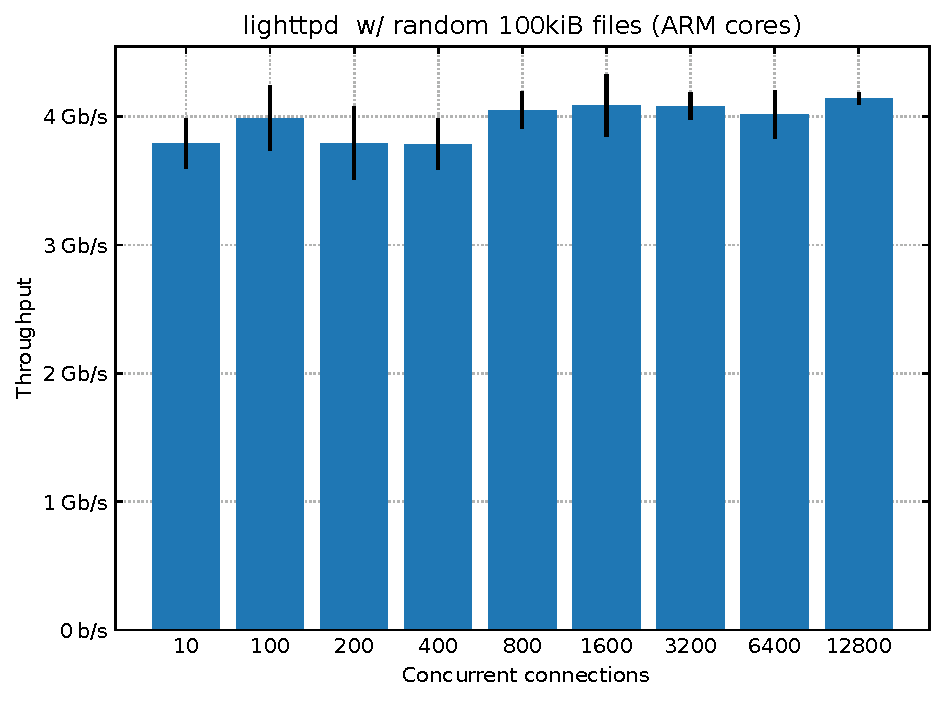
\includegraphics[width=\linewidth]{../measurements/npf/experiments/lighttpd/bluefield-random-100k-BANDWIDTH.pdf}
        \caption{Throughput of lighttpd on SmartNIC (ARM Cortex-A72 core)}
        \label{fig:lighttpd-arm}
    \end{minipage}
\end{figure}


\section{IO-TCP performances}


\section{Implementation performances}
